\documentclass{beamer}
\usetheme{manhattan}  % Now it's a beamer presentation with the Manhattan College theme!

\usepackage{url}
\usepackage{graphicx}
\usepackage{salgorithm}
\usepackage{verbatim}
\usepackage{amsthm, amsfonts, amsmath, amssymb, amsxtra}

\newcommand{\NP}{\ensuremath{\mathcal{NP}}}
% Make a new command that will make a new subsection and a frame with the same title
\newcommand{\fst}[2]{\subsection{#1}\frame{\frametitle{#1} #2}}

\title{Animation of Object-Oriented Program Execution}
\author{Peter Boothe}
\date{27 July 2011\\
BRIDGES 2011}
\institute[Manhattan College]{
    \url{peter.boothe@manhattan.edu}\\
    Mathematics and Computer Science \\
    Manhattan College}

\begin{document}
\frame{\titlepage}

\section{Why}

\fst{Beautiful programs}{
\begin{center}Programmers are beginning to talk about beauty

\uncover<2->{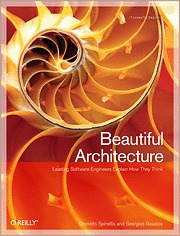
\includegraphics[width=.5in]{barch.jpg}}
\uncover<1->{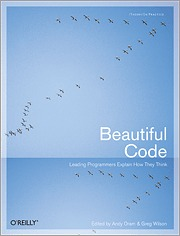
\includegraphics[width=.5in]{bcode.jpg}}
\uncover<5->{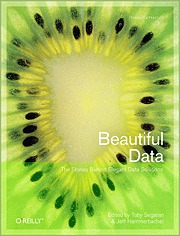
\includegraphics[width=.5in]{bdata.jpg}}
\uncover<4->{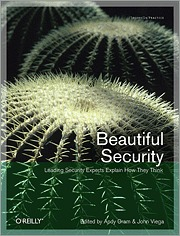
\includegraphics[width=.5in]{bsec.jpg}}
\uncover<3->{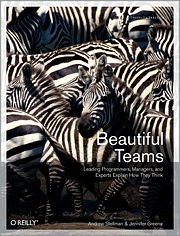
\includegraphics[width=.5in]{bteam.jpg}}
\uncover<6->{
\includegraphics[width=.5in]{btest.jpg}}
\uncover<7->{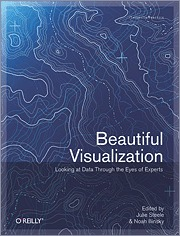
\includegraphics[width=.5in]{bvis.jpg}}
\end{center}

\uncover<7->{My claim:}
\uncover<8->{\LARGE \it The beauty of a program comes not from its source code, but from the unfolding of its execution.}
}

\fst{Programs are blueprints}{

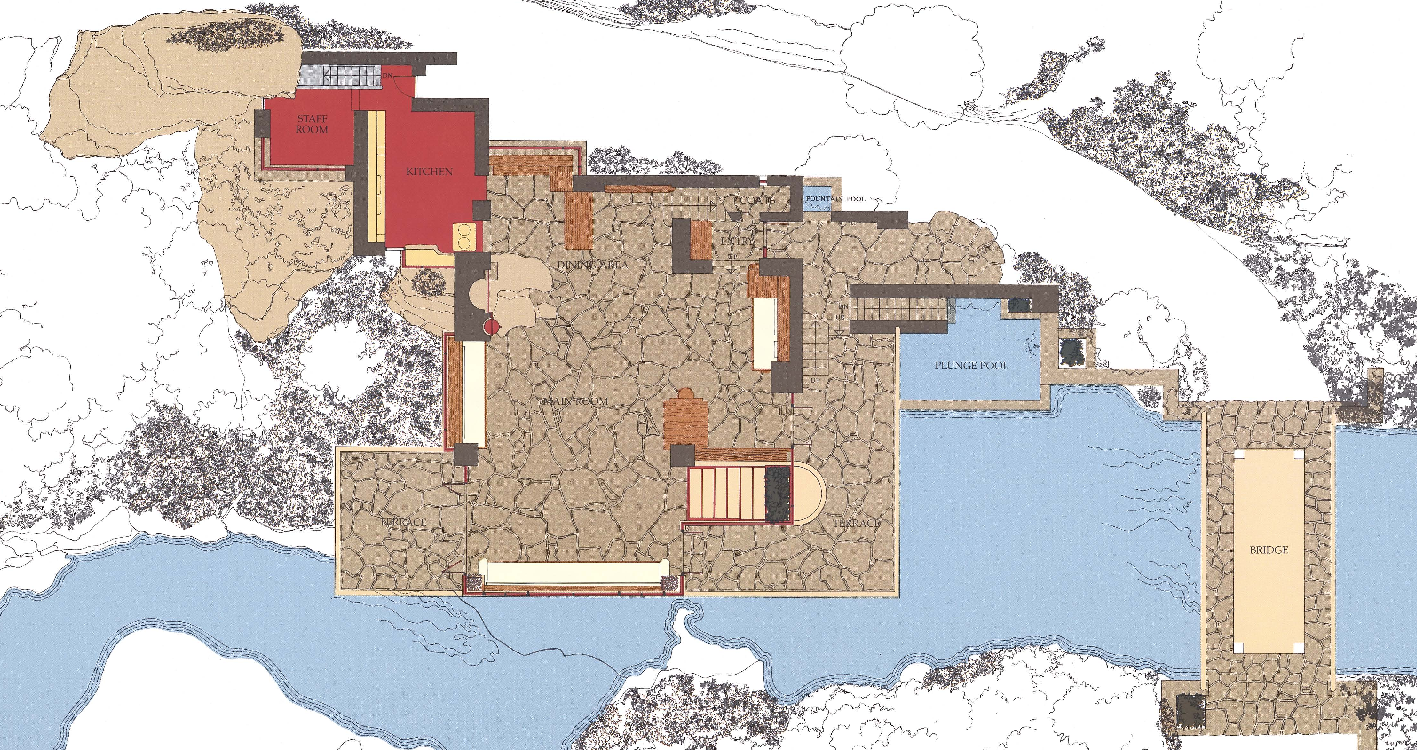
\includegraphics[width=4in]{fw.png}

}

\fst{The execution is what matters}{

\centering
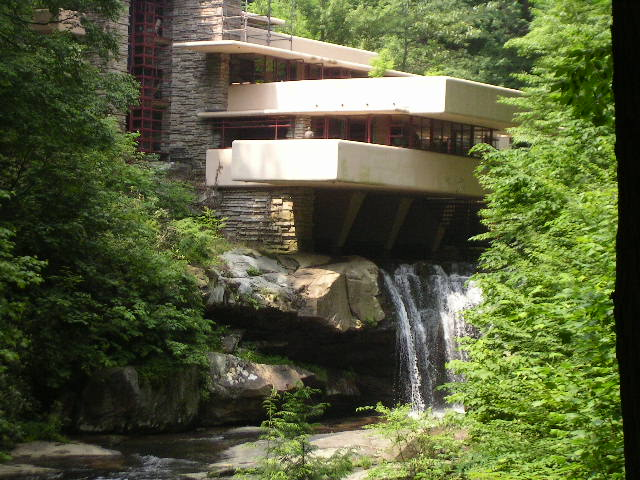
\includegraphics[width=3in]{fwpic.jpg}

{\tiny Thanks \url{http://www.fallingwater.org/assets/Site\%20Plan\%20and\%20Floor\%20Plans.pdf} and \url{http://www.flickr.com/photos/spike55151/14471574/}}
}

\section{Past Examples}

\fst{Algorithm Visualization}{
\begin{tabular}{c p{2in}}
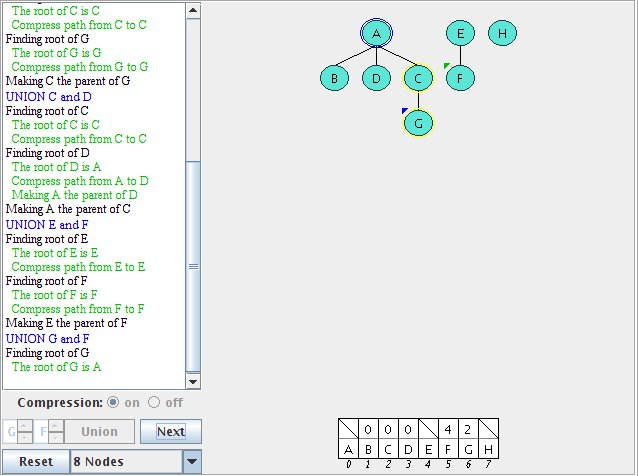
\includegraphics[width=2in]{algoviz.jpg} &
\vspace{-1.5in}
\begin{itemize}
\item Custom on a per-algorithm basis
\item Tricky to write
\item Not trying for beauty
\item Only one kind of beauty
\item Doesn't seem to help students learn
\end{itemize}
\end{tabular}

Many more at \url{http://algoviz.org}

Picture is from \url{http://research.cs.vt.edu/AVresearch/UF/} 
}

\subsection{Lisp}
\frame[containsverbatim]{
\frametitle{Lisp and Trees}
\centering
\begin{tabular}{p{2in} p{2in}}
\vspace{-1.85in}
\begin{verbatim}
(((fun (f) (f f) ) 
  (fun (f) 
    (fun (n) 
     (if (< n 2) 1
      (* n ((f f) (- n 1)))
     )
    )
   )
 ) 6)
\end{verbatim} 
& 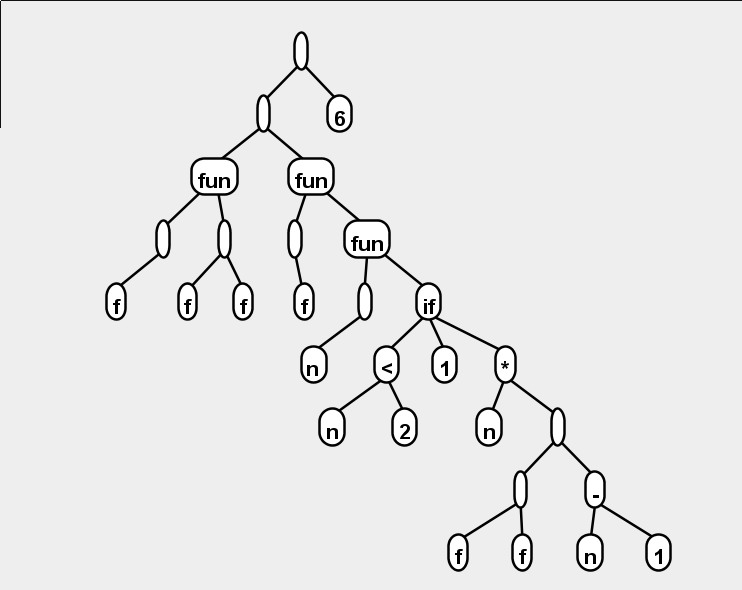
\includegraphics[width=2in]{fact.png} \\
\end{tabular}
}

\fst{Debuggers}{
\begin{center}
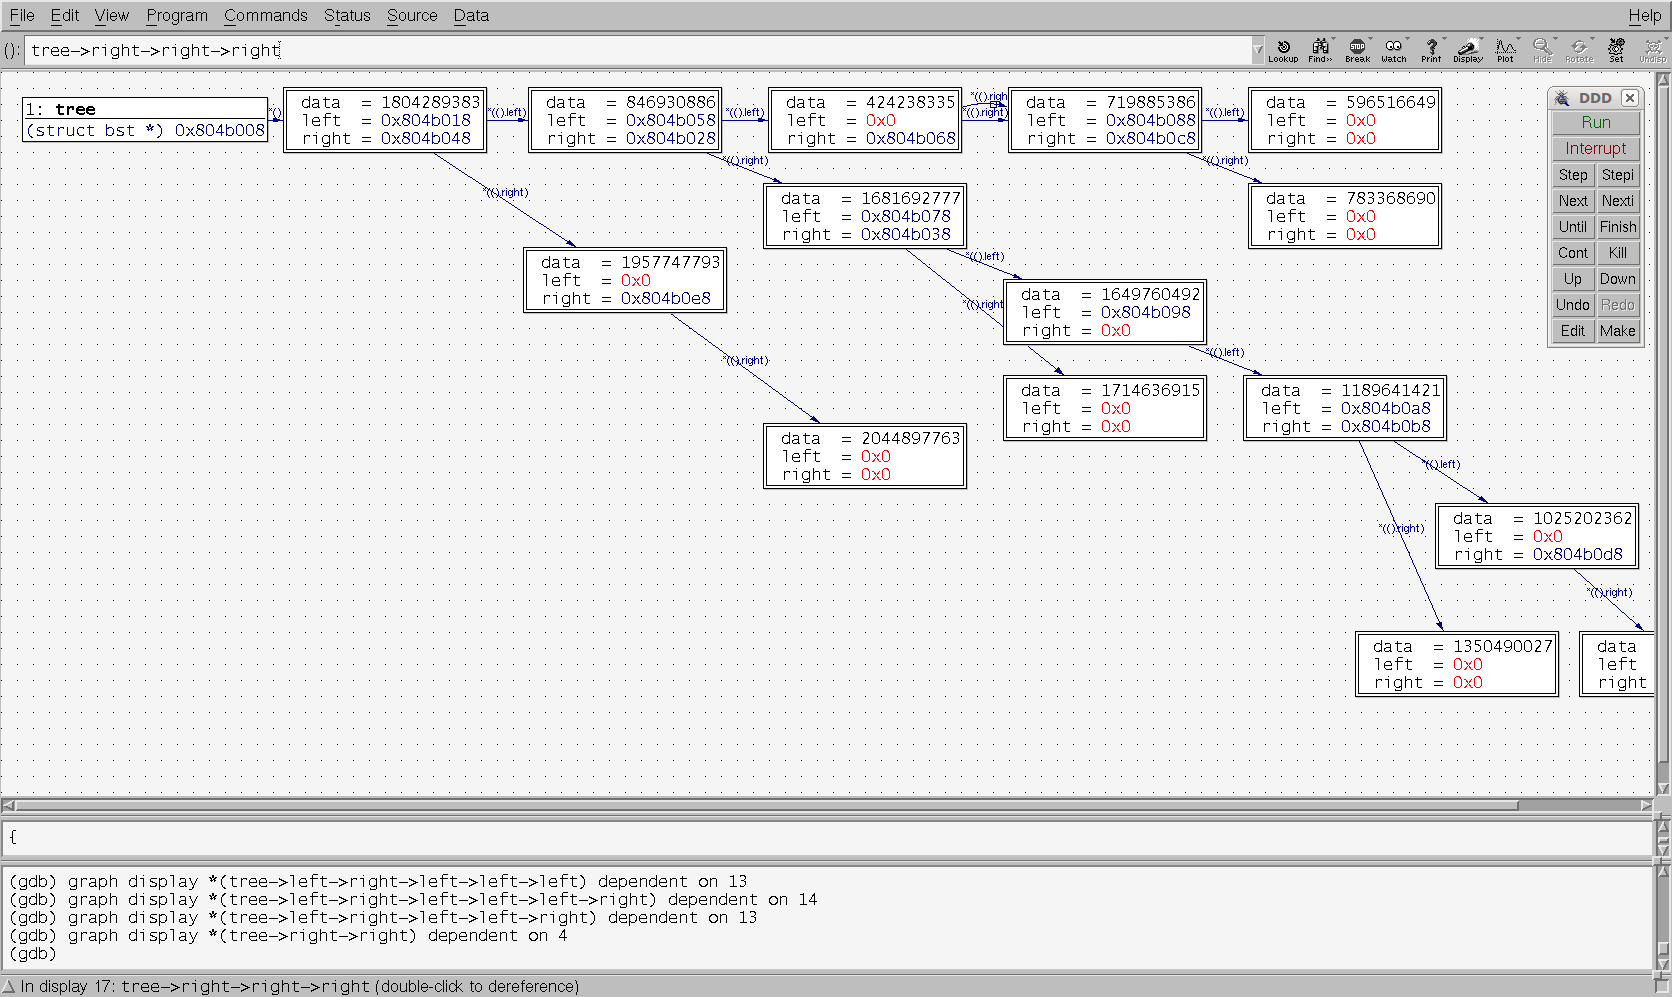
\includegraphics[width=4in]{ddd.png}
\end{center}
}

\fst{OO programs}{
}

\section{Programs $\to$ Graphs}

\fst{Use the debugger}{}

\section{Animating the program}

\fst{Lay it out}{}
\fst{Tween the states}{}
\fst{Animate it}{}

\section{Demo}

\fst{Demo}{Here are a few programs, to end my talk}

\end{document}
